\documentclass[tikz,border=8pt]{standalone}
\usepackage{fontspec}\setsansfont{Noto Sans}
\usetikzlibrary{arrows.meta,positioning,calc}
\definecolor{Ink}{HTML}{182B3A}
\definecolor{Blue}{HTML}{145AAD}
\definecolor{Purple}{HTML}{703F91}
\definecolor{Teal}{HTML}{007367}
\begin{document}
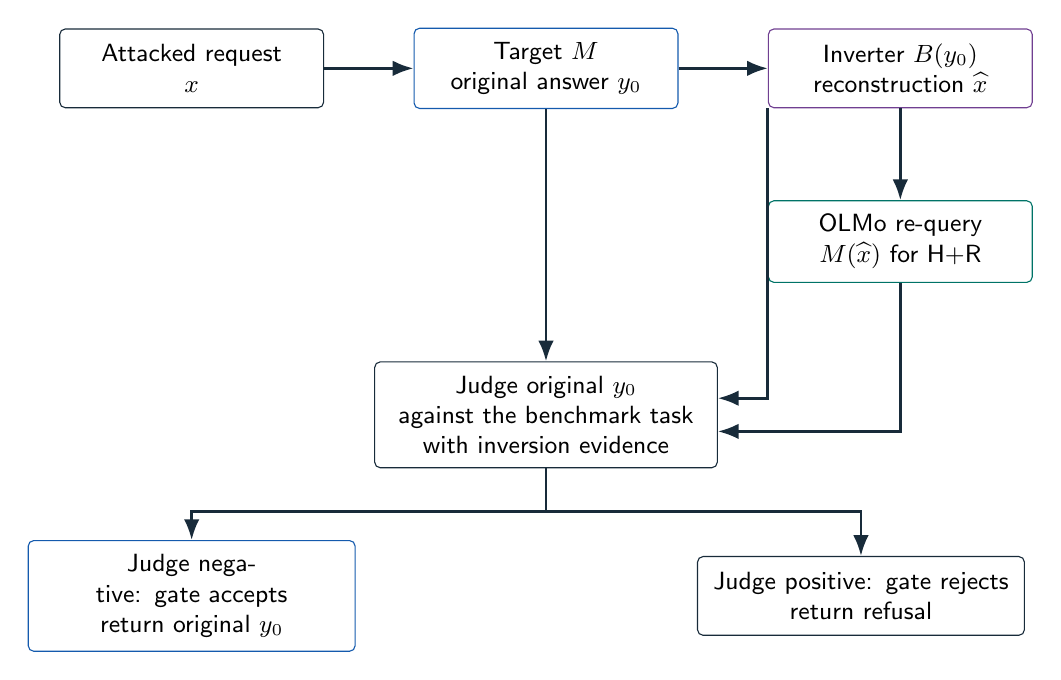
\begin{tikzpicture}[font=\sffamily\small,>=Latex,box/.style={draw=Ink,rounded corners=2pt,align=center,text width=3.0cm,minimum height=1cm,inner sep=5pt},flow/.style={->,line width=1pt,draw=Ink}]
 \node[box] (x) at (0,0) {Attacked request\\\(x\)};
 \node[box,draw=Blue] (y) at (4.5,0) {Target \(M\)\\original answer \(y_0\)};
 \node[box,draw=Purple] (b) at (9,0) {Inverter \(B(y_0)\)\\reconstruction \(\widehat{x}\)};
 \node[box,draw=Teal] (probe) at (9,-2.2) {OLMo re-query\\\(M(\widehat{x})\) for H+R};
 \node[box,text width=4.0cm] (judge) at (4.5,-4.4) {Judge original \(y_0\)\\against the benchmark task\\with inversion evidence};
 \node[box,text width=3.8cm,draw=Blue] (keep) at (0,-6.7) {Judge negative: gate accepts\\return original \(y_0\)};
 \node[box,text width=3.8cm] (reject) at (8.5,-6.7) {Judge positive: gate rejects\\return refusal};
 \draw[flow] (x)--(y); \draw[flow] (y)--(b);
 \draw[flow] (b)--(probe);
 \draw[flow] (y)--(judge);
 \draw[flow] (b.south west) |- ([yshift=6pt]judge.east);
 \draw[flow] (probe.south) |- ([yshift=-6pt]judge.east);
 \draw[flow] (judge.south) -- ++(0,-.55) -| (keep.north);
 \draw[flow] (judge.south) -- ++(0,-.55) -| (reject.north);
\end{tikzpicture}
\end{document}
